%%%%%%%%%%%%%%%%%%%%%%%%%%%%%%%%%%%%%%%%%%%%%%
%                                            %
%   W Z O R Z E C   S P R A W O Z D A N I A  %
%                                            %
%%%%%%%%%%%%%%%%%%%%%%%%%%%%%%%%%%%%%%%%%%%%%%


\documentclass[12pt,a4paper,twoside]{article}

\usepackage{amsmath,amssymb}
\usepackage[utf8]{inputenc}                                      
\usepackage[OT4]{fontenc}      
%\usepackage[T1]{fontenc}                            
\usepackage[polish]{babel}                           
\selectlanguage{polish}
\usepackage{indentfirst} 
\usepackage[dvips]{graphicx}
\usepackage{tabularx}
\usepackage{color}
\usepackage{hyperref} 
\usepackage{fancyhdr}
\usepackage{listings}
\usepackage{booktabs}
\usepackage{ifpdf}
\usepackage{mathtext} % polskie znaki w trybie matematycznym
%\makeindex  % utworzenie skorowidza (w dokumencie pdf)
\usepackage{lmodern}
%\usepackage[osf]{libertine}
\usepackage{filecontents}
\usepackage{ifthen}


\newcounter{nextYear}
\setcounter{nextYear}{\the\year}
\stepcounter{nextYear}

% rozszerzenie nieco strony
%\setlength{\topmargin}{-1cm} \setlength{\textheight}{24.5cm}
%\setlength{\textwidth}{17cm} \addtolength{\hoffset}{-1.5cm}
%\setlength{\parindent}{0.5cm} \setlength{\footskip}{2cm}
%\linespread{1.2} % odstep pomiedzy wierszami


%%%% ZYWA PAGINA %%%%%%%%%%%
\newcommand{\tl}[1]{\textbf{#1}} 
\pagestyle{fancy}
\renewcommand{\sectionmark}[1]{\markright{\thesection\ #1}}
\fancyhf{} % usuwanie bieżących ustawień
\fancyhead[LE,RO]{\small\bfseries\thepage}
\fancyhead[LO]{\small\bfseries\rightmark}
\fancyhead[RE]{\small\bfseries\leftmark}
\renewcommand{\headrulewidth}{0.5pt}
\renewcommand{\footrulewidth}{0pt}
\addtolength{\headheight}{0.5pt} % pionowy odstęp na kreskę
\fancypagestyle{plain}{%
\fancyhead{} % usuń p. górne na stronach pozbawionych numeracji
\renewcommand{\headrulewidth}{0pt} % pozioma kreska
}

%%%%%   LISTINGI %%%%%%%%
% ustawienia listingu programow

\lstset{%
language=C,%
commentstyle=\textit,%
identifierstyle=\textsf,%
keywordstyle=\sffamily\bfseries, %
%captionpos=b,%
tabsize=3,%
frame=lines,%
numbers=left,%
numberstyle=\tiny,%
numbersep=5pt,%
breaklines=true,%
morekeywords={pWezel,Wezel,string,ref,params_result},%
escapeinside={(*@}{@*)},%
%basicstyle=\footnotesize,%
%keywords={double,int,for,if,return,vector,matrix,void,public,class,string,%
%float,sizeof,char,FILE,while,do,const}
}
%%%%%%%%%%%%%%%%%%%%%%%%%%%%%%%%%%%%%%%%%%%%%%%%%%%%%%%%%%%%%%%%%%%%%%%

%%%%%%%%%  NOTKI NA MARGINESIE %%%%%%%%%%%%%

% % % % % % % % % % % % % % % % % % % % % % % % % % % % % % % %

%%%% WYSWIETLANIE AKTUALNEGO ROKU AKADEMICKIEGO %%%%%%%%%%%
\newcounter{rok}
\newcommand{\rokakademicki}{%
   \setcounter{rok}{\number\year}%
   \ifthenelse{\number\month<10}%
   {\addtocounter{rok}{-1}}% rok akademicki zaczal sie w pazdzierniku poprzedniego roku
   {}%                       rok akademicki zaczyna sie w pazdzierniku tego roku
   \arabic{rok}/\addtocounter{rok}{1}\arabic{rok}
}
%%%%%%%%%%%%%%%%%%%%%%%%%%%%%%%%%%%%%%%


%%%% LISTA UWAG %%%%%%%%%
\usepackage{color}
\definecolor{brickred}      {cmyk}{0   , 0.89, 0.94, 0.28}

\makeatletter \newcommand \kslistofremarks{\section*{Uwagi} \@starttoc{rks}}
\newcommand\l@uwagas[2]
{\par\noindent \textbf{#2:} %\parbox{10cm}
   {#1}\par} \makeatother


\newcommand{\ksremark}[1]{%
   {{\color{brickred}{[#1]}}}%
   \addcontentsline{rks}{uwagas}{\protect{#1}}%
}

\newcommand{\comma}{\ksremark{przecinek}}
\newcommand{\nocomma}{\ksremark{bez przecinka}}
\newcommand{\styl}{\ksremark{styl}}
\newcommand{\ortografia}{\ksremark{ortografia}}
\newcommand{\fleksja}{\ksremark{fleksja}}
\newcommand{\pauza}{\ksremark{pauza `--', nie dywiz `-'}}
\newcommand{\kolokwializm}{\ksremark{kolokwializm}}
\newcommand{\cytowanie}{\ksremark{cytowanie}}

%%%%%%%%%%%%%%%%%%%%%%%%%
%%%%%%%%%%%%%%%%%%%%%%%%%
%%%%%%%%%%%%%%%%%%%%%%%%%
%%%%%%%%%%%%%%%%%%%%%%%%%
%%%%%%%%%%%%%%%%%%%%%%%%%
%%%%%%%%%%%%%%%%%%%%%%%%%
%%%%%%%%%%%%%%%%%%%%%%%%%
%%%%%%%%%%%%%%%%%%%%%%%%%
%%%%%%%%%%%%%%%%%%%%%%%%%
%%%%%%%%%%%%%%%%%%%%%%%%%
%%%%%%%%%%%%%%%%%%%%%%%%%
%%%%%%%%%%%%%%%%%%%%%%%%%



% autor:
\fancyhead[RE]{\small\bfseries Aleksander Augustyniak} % autor sprawozdania



%%%%%%%%%%% NO I ZACZYNA SIE SPRAWOZDANIE %%%%%%%%%%%

\begin{document}
\frenchspacing
\thispagestyle{empty}
\begin{center}
{\Large\sf Politechnika Śląska   % Alma Mater

Wydział Automatyki, Elektroniki i Informatyki

}

\vfill

 

\vfill\vfill

{\Huge\sffamily\bfseries Programowanie Komputerów\par}  

\vfill\vfill

{\LARGE\sf Operacje morfologiczne na obrazie}   


\vfill \vfill\vfill\vfill

%%%%%%%%%%%%%%%%%%%%%%%%%%%%





\begin{tabular}{ll}
	\toprule
	autor                       & Aleksander Augustyniak     \\
	prowadzący                  & mgr inż. Marek Kokot  \\
	rok akademicki              & \rokakademicki         \\
	kierunek                    & informatyka            \\
	rodzaj studiów              & SSI                    \\
	semestr                     & 2                      \\
	termin laboratorium         & środa, 11:30 – 13:00 \\
	sekcja                      & druga                     \\
	termin oddania sprawozdania & 2020-09-18             \\
	\bottomrule
	                            &
\end{tabular}

\end{center}
%%% koniec strony  tytulowej

%%%%%%%%%%%%%%%%%%%%%%%%%%%%%%%%%%%%%%%%%%%%%%%%%%%%%%%%%%%%%%%%%%%%%%%%%
\cleardoublepage
%%%%%%%%%%%%%%%%%%%%%%%%%%%%%%%%%%%%%%%%%%%%%%%%%%%%%%%%%%%%%%%%%%%%%%%%%

%%%%%%%%%%%%%%%%%%%%%%%%%%%%%%%%%%%%%%%%%%%%%%%%%%%%%%%%%%%%%%%%%%%%%%%%%
\section{Treść zadania}
%\marginpar{Dokładny opis zadania, zgodny z tematem podanym przez prowadzącego.}
Napisać program umożliwiający przeprowadzenie operacji morfologicznych obrazu zawartego w pliku BMP. Element strukturalny powinien być zdefiniowany przez użytkownika poprzez dostarczenie odpowiedniego pliku tekstowego. Program powinien działać dla obrazów czarno-białych. Program
powinien umożliwić wykonanie następujących operacji: dylatacji, erozji, otwarcia oraz domknięcia. \cite{id:BMPWiki}

%%%%%%%%%%%%%%%%%%%%%%%%%%%%%%%%%%%%%%%%%%%%%%%%%%%%%%%%%%%%%%%%%%%%%%%%%
\section{Analiza zadania}

Zadanie polega na cyfrowej obróbce czarno-białego obrazu, używając operacji morfologicznych, które tworzą podstawę zaawansowanych systemów rozpoznających kształty, odległości pomiędzy figurami, szkielet danego kształtu, etc. \par
Biorąc pod uwagę, że w obrazie występują wyłącznie dwa kolory (biały i czarny), dla ułatwienia i skrócenia pisowni można danym pikselom przypisać binarny stan, w którym się znajdują. Piksel czarny można oznaczyć binarnym \emph{0} - ze względu na zerowe składowe kolorów, z których się składa; oraz - analogicznie – piksel biały, jako binarne \emph{1} ze względu na maksymalną, posiadaną przezeń wartość poszczególnych składowych koloru. \par
Pracując nad projektem, w którym występują dwa kolory, można wprowadzić założenie, że kolor czarny reprezentuje pierwszy plan, a biały – tło.


\subsection{Element strukturalny}

Warunkowanie wykonania odpowiedniej modyfikacji na pikselach obrazu następuje przy pomocy elementu strukturalnego – maski, która jest \emph{przykładana} do każdego z nich w sposób zgodny z punktem głównym elementu strukturalnego. Element strukturalny posiada tylko jeden punkt główny. Ponadto posiada również informacje o tym, które punkty względem punktu głównego podlegają sprawdzeniu na obrazie. \par

\begin{figure}[hbt!]
  \centering
  
\includegraphics[width=0.5\textwidth]{grafika1.png}
  \caption{Najpopularniejsze elementy strukturalne. Od lewej – element strukturalny o sąsiedztwie czterospójnym (von Neumanna) i ośmiospójne (Moore'a) –  osiem pikseli sąsiaduje z punktem głównym elementu strukturalnego.}  \label{fig:grafika1}
\end{figure}

\begin{figure}[hbt!]
  \centering
  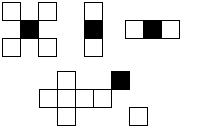
\includegraphics[width=0.5\textwidth]{grafika2.png}
  \caption{Inne, niestandardowe elementy strukturalne.}  \label{fig:grafika2}
\end{figure}


\clearpage
	
\subsection{Struktury danych}

Plik BMP jest plikiem binarnym, którego bajty są usytuowane w odpowiedniej kolejności. Taką strukturę można nazwać stałą, bądź statyczną – rozmiary poszczególnych zawartości są z góry ustalone i nie podlegają jakiejkolwiek zmianie. Jakakolwiek zmiana kolejności spowodowałoby trwałe uszkodzenie pliku.
\begin{figure}[hbt!]
\begin{center}
\begin{tabular} { |c|l|c| } 
\hline
 Numer bajtu & Zawartość & Rozmiar [$B$] \\ 
 \hline
 0  & Pierwsza litera identyfikatora pliku. & 1 \\ 
 1  & Druga litera identyfikatora pliku. & 1 \\ 
 2  & Rozmiar całego pliku. & 4 \\
 6  & Zarezerwowany dla innych aplikacji. & 4 \\
 10  & Numer bajtu, który zaczyna macierz. & 2 \\
 14 & Rozmiar struktury nagłówka DIB. & 4 \\
 18 & Szerokość obrazu. & 4 \\
 22 & Wysokość obrazu. & 4 \\
 26 & Liczba płaszczyzn kolorów. & 2 \\
 28 & Ilość bitów na piksel. & 2 \\
 30 & Metoda kompresji. & 4 \\
 34 & Powierzchnia obrazu. & 4 \\
 38 & Rozdzielczość pozioma. & 4 \\
 42 & Rozdzielczość pionowa. & 4 \\
 46 & Ilość kolorów w palecie. & 4 \\
 50 & Ilość ważnych kolorów w palecie. & 1 \\
 51 & Flaga wyznaczająca, czy ma nastąpić rotacja palet. & 1 \\
 52 & — & 2 \\
 \hline
\end{tabular}
\caption{Ułożenie struktury nagłówka pliku i nagłówka DIB w pliku o rozszerzeniu BMP.} \label{tab:tab1}
\end{center}
\end{figure}
\\
Oprócz tego, program przechowuje dane posługując się m.in. dynamiczną listą jednokierunkową (w której przechowywany jest element strukturalny). \par



\subsection{Algorytmy}

Program składa się z nietrudnych algorytmów. Ich złożoność zwiększa się proporcjonalnie co do wielkości elementu strukturalnego i wielkości obrazu, który poddajemy obróbce. Sczytując piksele obrazu wejściowego, program \textit{sprawdza}, czy wszystkie składowe koloru piksela, w danej chwili sprawdzanego przez program, są równe zeru, jeżeli tak - żadna modyfikacja nie jest podejmowana - w przeciwnym wypadku wszystkie składowe są zwiększane do maksymalnej wartości. \par
Istotnym - w zasadzie najważniejszym - algorytmem jest algorytm \textit{sprawdzający} sąsiedztwo piksela modyfikowanego i warunkujący, czy ów piksel ma zostać zmodyfikowany. Algorytm ten działa na zasadzie \textit{przykładania} elementu strukturalnego do każdego, pojedynczego piksela obrazu i porównywania z otaczającymi piksel modyfikowany pikselami.


%%%%%%%%%%%%%%%%%%%%%%%%%%%%%%%%%%%%%%%%%%%%%%%%%%%%%%%%%%%%%%%%%%%%%%%%%
\section{Specyfikacja zewnętrzna}
\label{sec:sp:zewnetrzna}


Aby uruchomić program należy podać dokładne lokalizacje odpowiednich plików w linii poleceń w odpowiedniej kolejności, oddzielając poszczególne argumenty znakiem spacji: \par

\begin{tabular}{l}
\texttt {input output sieve char} 
\end{tabular}

Gdzie: \\
\texttt {input} - obraz wejściowy o rozszerzeniu BMP. \\
\texttt {output} - obraz wyjściowy o rozszerzeniu BMP. \\
\texttt {sieve} - plik tekstowy, zawierający element strukturalny (o rozszerzeniu TXT). \\
\texttt {char} - znak operacji morfologicznej, która ma zostać wykonana. \par
Plik tekstowy, zawierający element strukturalny musi spełniać pewne założenia:
\begin{itemize}
\item Zawierać punkt główny, oznaczany małą literą \emph{o}. W przypadku, gdy plik tekstowy zawiera więcej, niż jeden punkt główny, następne wystąpienia będą traktowane jak punkt sąsiedni punktu głównego.
\item Zawierać przynajmniej jeden punkt sąsiedni, oznaczany \emph{-} znakiem minus.
\end{itemize}
Niedostosowanie się do przynajmniej jednego z warunków skutkuje zakończeniem pracy programu i wyjściem. \\
Przykładowa zawartość pliku tekstowego zawierającego element strukturalny.

\begin{center}
\begin{tabular}{ccc}
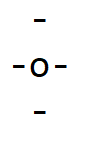
\includegraphics[scale=1]{grafika3}
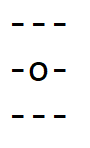
\includegraphics[scale=1]{grafika4}
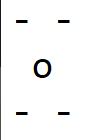
\includegraphics[scale=1]{grafika5}
\end{tabular}
\end{center}

Program, sczytując poszczególne, podane przez użytkownika argumenty, sprawdza, czy każdy z plików rzeczywiście istnieje, i czy dostęp do niego nie jest niemożliwy do uzyskania. Jeżeli przynajmniej jeden z plików nie zostanie wczytany do pamięci programu, program kończy swoją pracę wypisując odpowiedni kod błędu. \par

Kody błędów:
\begin{itemize}
\item 98 - Do programu nie została dostarczona wystarczająca ilość argumentów do poprawnego działania.
\item 99 - Wczytany plik wejściowy nie jest plikiem mapy bitowej.
\item 100 - Nie udało się wczytać elementu strukturalnego.
\item 101 - Nie udało się otworzyć pliku wejściowego.
\item 102, 103 - Nie udało się poprawnie wczytać nagłówka pliku.
\item 104 - Nie udało się zarezerwować odpowiedniej ilości pamięci dla struktury elementu strukturalnego.
\item 105 - Nie udało się zagospodarować odpowiedniej ilości pamięci dla współrzędnych punktu modyfikowanego (piksela modyfikowanego).
\item 106 - Nie udało się zaalokować wymaganej ilości pamięci do przechowania skłądowych koloru poszczególnych pikseli pliku wejściowego.
\item 107 - Nie udało się zaalokować wymaganej ilości pamięci do przechowania skłądowych koloru poszczególnych pikseli pliku wyjściowego.
\item 108 - Nie udało się utworzyć, bądź otworzyć istniejący plik wejściowy.
\end{itemize}



%%%%%%%%%%%%%%%%%%%%%%%%%%%%%%%%%%%%%%%%%%%%%%%%%%%%%%%%%%%%%%%%%%%%%%%%%
\section{Specyfikacja wewnętrzna oraz szczegółowy opis typów i funkcji}\label{sec:sp-wew}
Szczegółowy opis typów i funkcji znajduje się w załączniku.

\subsection{Ogólna struktura programu}
%\marginpar{Ogólna struktura programu, żeby czytelnik miał rozeznanie, co się w programie dzieje, jak program jest skonstruowany.}

Program realizuje funkcje w odpowiedniej kolejności:
\begin{enumerate}
\item Sprawdzenie, czy została podana odpowiednia ilość argumentów.
\item Otwarcie pliku wejściowego.
\item Załadowanie do struktury nagłówka pliku wejściowego w celu odczytania kluczowych danych,, tj. sprawdzenie, czy plik wejściowy jest plikiem mapy bitowej.
\item Otwarcie pliku, zawierającego element strukturalny.
\item Wczytanie elementu strukturalnego do struktury elementu strukturalnego.
\item Zapisanie do pamięci współrzędnych piksela modyfikowanego.
\item Zajęcie odpowiedniej ilości pamięci na obraz wyjściowy.
\item Wykonanie operacji morfologicznej i zapisanie wyniku do struktury wyjściowej.
\item Przepisanie danych z nagłówka pliku wejściowego do nagłówka pliku wyjściowego.
\item Zwolnienie całej pamięci zajętej przez program.
\end{enumerate}

\section{Testowanie}
%\marginpar{Należy opisać jak program był testowany (na zbiorach poprawnych i typowych, na zbiorach poprawnych, ale nietypowych i wreszcie na zbiorach niepoprawnych). Należy opisać zbiory testowe.}
Program został przetestowany na obrazach różnorakich – tych spełniających założenia zadania, jak i tych, które nie do końca pokrywają się z wymaganiami (lecz nieuszkodzonymi). Testy były wykonane na obrazach o dużej powierzchni pikseli. \\

Program został sprawdzony pod kątem wycieków pamięci. \\

Program przetestowany na komputerze z systemem Windows 10.

\clearpage

\subsection{Wyniki}
Poniżej przedstawione zostały wyniki programu dla sześciu różnych elementów strukturalnych i trzech różnych obrazów wejściowych. \\
W lewym górnym rogu: erozja. \\
W prawym górnym rogu: dylatacja. \\
W lewym dolnym rogu: otwarcie. \\
W prawym dolnym rogu: domknięcie. \\


\begin{figure}[h!]
\fbox{\centering 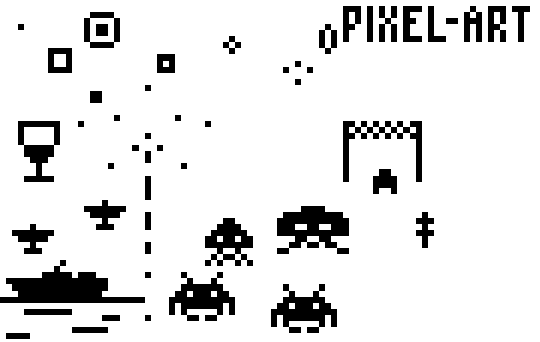
\includegraphics[width=\textwidth,keepaspectratio=true]{testowanie/sample1.png}} \\
\caption{Obraz wejściowy numer 1.} 
\end{figure}

\begin{figure}[h!]
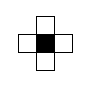
\includegraphics[scale=.5]{sieve1.png} \\
\fbox{
\includegraphics[width=0.33\textwidth,keepaspectratio=true]{testowanie/erozja1/wynik1.png}}
\fbox{
\includegraphics[width=0.33\textwidth,keepaspectratio=true]{testowanie/dylatacja1/wynik1.png}} \\
\fbox{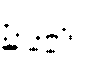
\includegraphics[width=0.33\textwidth,keepaspectratio=true]{testowanie/otwarcie1/wynik1.png}}
\fbox{
\includegraphics[width=0.33\textwidth,keepaspectratio=true]{testowanie/zamkniecie1/wynik1.png}} \\
\end{figure}

\begin{figure}[h!]

\includegraphics[scale=.5]{sieve2.png} \\
\fbox{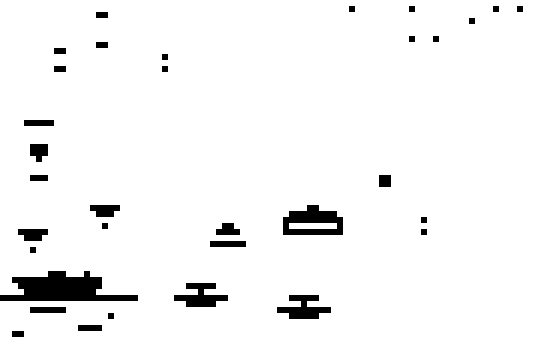
\includegraphics[width=0.33\textwidth,keepaspectratio=true]{testowanie/erozja1/wynik2.png}}
\fbox{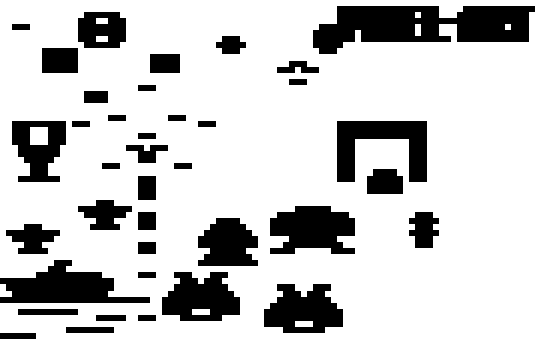
\includegraphics[width=0.33\textwidth,keepaspectratio=true]{testowanie/dylatacja1/wynik2.png}} \\
\fbox{
\includegraphics[width=0.33\textwidth,keepaspectratio=true]{testowanie/otwarcie1/wynik2.png}}
\fbox{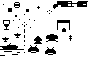
\includegraphics[width=0.33\textwidth,keepaspectratio=true]{testowanie/zamkniecie1/wynik2.png}} \\
\end{figure}

\begin{figure}[h!]
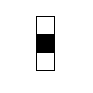
\includegraphics[scale=.5]{sieve3.png} \\
\fbox{
\includegraphics[width=0.33\textwidth,keepaspectratio=true]{testowanie/erozja1/wynik3.png}}
\fbox{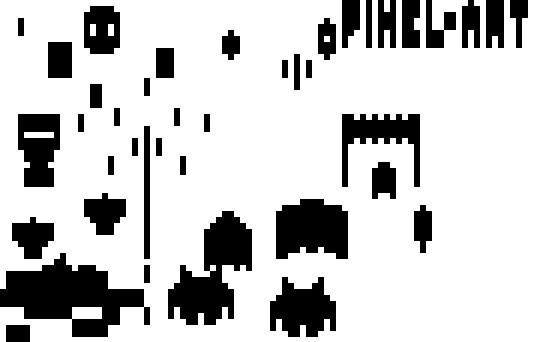
\includegraphics[width=0.33\textwidth,keepaspectratio=true]{testowanie/dylatacja1/wynik3.png}} \\
\fbox{
\includegraphics[width=0.33\textwidth,keepaspectratio=true]{testowanie/otwarcie1/wynik3.png}}
\fbox{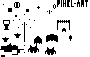
\includegraphics[width=0.33\textwidth,keepaspectratio=true]{testowanie/zamkniecie1/wynik3.png}} \\
\end{figure}

\begin{figure}[h!]
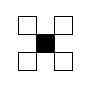
\includegraphics[scale=.5]{sieve4.png} \\
\fbox{
\includegraphics[width=0.33\textwidth,keepaspectratio=true]{testowanie/erozja1/wynik4.png}}
\fbox{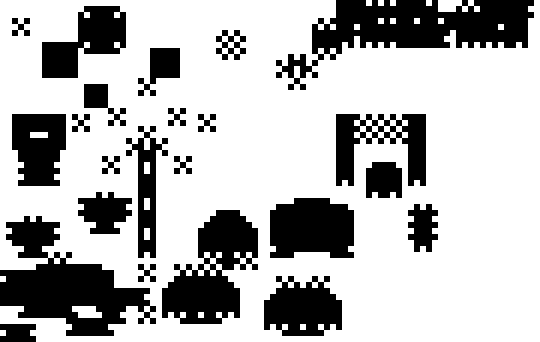
\includegraphics[width=0.33\textwidth,keepaspectratio=true]{testowanie/dylatacja1/wynik4.png}} \\
\fbox{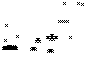
\includegraphics[width=0.33\textwidth,keepaspectratio=true]{testowanie/otwarcie1/wynik4.png}}
\fbox{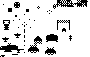
\includegraphics[width=0.33\textwidth,keepaspectratio=true]{testowanie/zamkniecie1/wynik4.png}} \\
\end{figure}

\begin{figure}[h!]
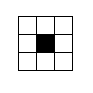
\includegraphics[scale=.5]{sieve5.png} \\
\fbox{
\includegraphics[width=0.33\textwidth,keepaspectratio=true]{testowanie/erozja1/wynik5.png}}
\fbox{
\includegraphics[width=0.33\textwidth,keepaspectratio=true]{testowanie/dylatacja1/wynik5.png}} \\
\fbox{
\includegraphics[width=0.33\textwidth,keepaspectratio=true]{testowanie/otwarcie1/wynik5.png}}
\fbox{
\includegraphics[width=0.33\textwidth,keepaspectratio=true]{testowanie/zamkniecie1/wynik5.png}} \\
\end{figure}

\begin{figure}[h!]
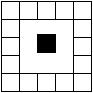
\includegraphics[scale=.5]{sieve6.png} \\
\fbox{
\includegraphics[width=0.33\textwidth,keepaspectratio=true]{testowanie/erozja1/wynik6.png}}
\fbox{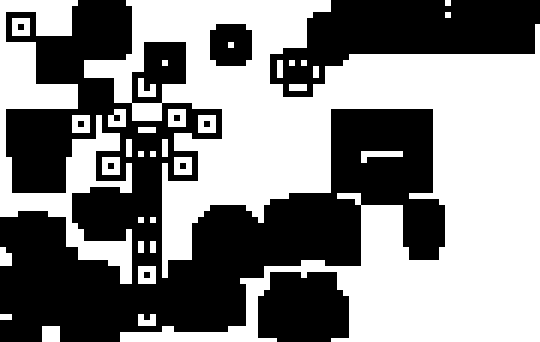
\includegraphics[width=0.33\textwidth,keepaspectratio=true]{testowanie/dylatacja1/wynik6.png}} \\
\fbox{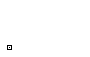
\includegraphics[width=0.33\textwidth,keepaspectratio=true]{testowanie/otwarcie1/wynik6.png}}
\fbox{
\includegraphics[width=0.33\textwidth,keepaspectratio=true]{testowanie/zamkniecie1/wynik6.png}} \\
\end{figure}


\begin{figure}[h!]
\fbox{\centering 
\includegraphics[width=\textwidth,keepaspectratio=true]{testowanie/sample2.png}} \\
\caption{Obraz wejściowy numer 2.} 
\end{figure}

\begin{figure}[h!]
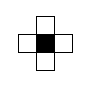
\includegraphics[scale=.5]{sieve1.png} \\
\fbox{
\includegraphics[width=0.33\textwidth,keepaspectratio=true]{testowanie/erozja2/wynik1.png}}
\fbox{
\includegraphics[width=0.33\textwidth,keepaspectratio=true]{testowanie/dylatacja2/wynik1.png}} \\
\fbox{
\includegraphics[width=0.33\textwidth,keepaspectratio=true]{testowanie/otwarcie2/wynik1.png}}
\fbox{
\includegraphics[width=0.33\textwidth,keepaspectratio=true]{testowanie/zamkniecie2/wynik1.png}} \\
\end{figure}

\begin{figure}[h!]

\includegraphics[scale=.5]{sieve2.png} \\
\fbox{
\includegraphics[width=0.33\textwidth,keepaspectratio=true]{testowanie/erozja2/wynik2.png}}
\fbox{
\includegraphics[width=0.33\textwidth,keepaspectratio=true]{testowanie/dylatacja2/wynik2.png}} \\
\fbox{
\includegraphics[width=0.33\textwidth,keepaspectratio=true]{testowanie/otwarcie2/wynik2.png}}
\fbox{
\includegraphics[width=0.33\textwidth,keepaspectratio=true]{testowanie/zamkniecie2/wynik2.png}} \\
\end{figure}

\begin{figure}[h!]
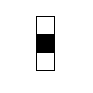
\includegraphics[scale=.5]{sieve3.png} \\
\fbox{
\includegraphics[width=0.33\textwidth,keepaspectratio=true]{testowanie/erozja2/wynik3.png}}
\fbox{
\includegraphics[width=0.33\textwidth,keepaspectratio=true]{testowanie/dylatacja2/wynik3.png}} \\
\fbox{\includegraphics[width=0.33\textwidth,keepaspectratio=true]{testowanie/otwarcie2/wynik3.png}}
\fbox{\includegraphics[width=0.33\textwidth,keepaspectratio=true]{testowanie/zamkniecie2/wynik3.png}} \\
\end{figure}

\begin{figure}[h!]
\includegraphics[scale=.5]{sieve4.png} \\
\fbox{\includegraphics[width=0.33\textwidth,keepaspectratio=true]{testowanie/erozja2/wynik4.png}}
\fbox{\includegraphics[width=0.33\textwidth,keepaspectratio=true]{testowanie/dylatacja2/wynik4.png}} \\
\fbox{\includegraphics[width=0.33\textwidth,keepaspectratio=true]{testowanie/otwarcie2/wynik4.png}}
\fbox{\includegraphics[width=0.33\textwidth,keepaspectratio=true]{testowanie/zamkniecie2/wynik4.png}} \\
\end{figure}

\begin{figure}[h!]
\includegraphics[scale=.5]{sieve5.png} \\
\fbox{\includegraphics[width=0.33\textwidth,keepaspectratio=true]{testowanie/erozja2/wynik5.png}}
\fbox{\includegraphics[width=0.33\textwidth,keepaspectratio=true]{testowanie/dylatacja2/wynik5.png}} \\
\fbox{\includegraphics[width=0.33\textwidth,keepaspectratio=true]{testowanie/otwarcie2/wynik5.png}}
\fbox{\includegraphics[width=0.33\textwidth,keepaspectratio=true]{testowanie/zamkniecie2/wynik5.png}} \\
\end{figure}

\begin{figure}[h!]
\includegraphics[scale=.5]{sieve6.png} \\
\fbox{\includegraphics[width=0.33\textwidth,keepaspectratio=true]{testowanie/erozja2/wynik6.png}}
\fbox{\includegraphics[width=0.33\textwidth,keepaspectratio=true]{testowanie/dylatacja2/wynik6.png}} \\
\fbox{\includegraphics[width=0.33\textwidth,keepaspectratio=true]{testowanie/otwarcie2/wynik6.png}}
\fbox{\includegraphics[width=0.33\textwidth,keepaspectratio=true]{testowanie/zamkniecie2/wynik6.png}} \\
\end{figure}

\begin{figure}[h!]
\fbox{\centering \includegraphics[width=\textwidth,keepaspectratio=true]{testowanie/sample3.png}} \\
\caption{Obraz wejściowy numer 3.} 
\end{figure}

\begin{figure}[h!]
\includegraphics[scale=.5]{sieve1.png} \\
\fbox{\includegraphics[width=0.33\textwidth,keepaspectratio=true]{testowanie/erozja3/wynik1.png}}
\fbox{\includegraphics[width=0.33\textwidth,keepaspectratio=true]{testowanie/dylatacja3/wynik1.png}} \\
\fbox{\includegraphics[width=0.33\textwidth,keepaspectratio=true]{testowanie/otwarcie3/wynik1.png}}
\fbox{\includegraphics[width=0.33\textwidth,keepaspectratio=true]{testowanie/zamkniecie3/wynik1.png}} \\
\end{figure}

\begin{figure}[h!]
\includegraphics[scale=.5]{sieve2.png} \\
\fbox{\includegraphics[width=0.33\textwidth,keepaspectratio=true]{testowanie/erozja3/wynik2.png}}
\fbox{\includegraphics[width=0.33\textwidth,keepaspectratio=true]{testowanie/dylatacja3/wynik2.png}} \\
\fbox{\includegraphics[width=0.33\textwidth,keepaspectratio=true]{testowanie/otwarcie3/wynik2.png}}
\fbox{\includegraphics[width=0.33\textwidth,keepaspectratio=true]{testowanie/zamkniecie3/wynik2.png}} \\
\end{figure}

\begin{figure}[h!]
\includegraphics[scale=.5]{sieve3.png} \\
\fbox{\includegraphics[width=0.33\textwidth,keepaspectratio=true]{testowanie/erozja3/wynik3.png}}
\fbox{\includegraphics[width=0.33\textwidth,keepaspectratio=true]{testowanie/dylatacja3/wynik3.png}} \\
\fbox{\includegraphics[width=0.33\textwidth,keepaspectratio=true]{testowanie/otwarcie3/wynik3.png}}
\fbox{\includegraphics[width=0.33\textwidth,keepaspectratio=true]{testowanie/zamkniecie3/wynik3.png}} \\
\end{figure}

\begin{figure}[h!]
\includegraphics[scale=.5]{sieve4.png} \\
\fbox{\includegraphics[width=0.33\textwidth,keepaspectratio=true]{testowanie/erozja3/wynik4.png}}
\fbox{\includegraphics[width=0.33\textwidth,keepaspectratio=true]{testowanie/dylatacja3/wynik4.png}} \\
\fbox{\includegraphics[width=0.33\textwidth,keepaspectratio=true]{testowanie/otwarcie3/wynik4.png}}
\fbox{\includegraphics[width=0.33\textwidth,keepaspectratio=true]{testowanie/zamkniecie3/wynik4.png}} \\
\end{figure}

\begin{figure}[h!]
\includegraphics[scale=.5]{sieve5.png} \\
\fbox{\includegraphics[width=0.33\textwidth,keepaspectratio=true]{testowanie/erozja3/wynik5.png}}
\fbox{\includegraphics[width=0.33\textwidth,keepaspectratio=true]{testowanie/dylatacja3/wynik5.png}} \\
\fbox{\includegraphics[width=0.33\textwidth,keepaspectratio=true]{testowanie/otwarcie3/wynik5.png}}
\fbox{\includegraphics[width=0.33\textwidth,keepaspectratio=true]{testowanie/zamkniecie3/wynik5.png}} \\
\end{figure}

\begin{figure}[h!]
\includegraphics[scale=.5]{sieve6.png} \\
\fbox{\includegraphics[width=0.33\textwidth,keepaspectratio=true]{testowanie/erozja3/wynik6.png}}
\fbox{\includegraphics[width=0.33\textwidth,keepaspectratio=true]{testowanie/dylatacja3/wynik6.png}} \\
\fbox{\includegraphics[width=0.33\textwidth,keepaspectratio=true]{testowanie/otwarcie3/wynik6.png}}
\fbox{\includegraphics[width=0.33\textwidth,keepaspectratio=true]{testowanie/zamkniecie3/wynik6.png}} \\
\end{figure}

\clearpage
%%%%%%%%%%%%%%%%%%%%%%%%%%%%%%%%%%%%%%%%%%%%%%%


% & \includegraphics[width=0.5\textwidth,keepaspectratio=true]{testowanie/erozja1/wynik1.png} \\

% \includegraphics[height=0.16\textheight]{sieve2.png} & \includegraphics[height=0.16\textheight,keepaspectratio=true]{testowanie/erozja1/wynik2.png} \\

% \includegraphics[height=0.16\textheight]{sieve3.png} & \includegraphics[height=0.16\textheight,keepaspectratio=true]{testowanie/erozja1/wynik3.png} \\

% \includegraphics[height=0.16\textheight]{sieve4.png} & \includegraphics[height=0.16\textheight,keepaspectratio=true]{testowanie/erozja1/wynik4.png} \\

% \includegraphics[height=0.16\textheight]{sieve5.png} & \includegraphics[height=0.16\textheight,keepaspectratio=true]{testowanie/erozja1/wynik5.png} \\

% \includegraphics[height=0.16\textheight]{sieve6.png} & \includegraphics[height=0.16\textheight,keepaspectratio=true]{testowanie/erozja1/wynik6.png} \\




\section{Wnioski}
Napisanie programu, który wykonuje podstawowe operacje morfologiczne należało do prostych. Nie miałem trudności z analizą zadania, ze względu na łatwość w niemalże natychmiastowym zauważeniu efektów pracy. Zadany temat uważam za bardzo interesujący ze względu na możliwe wykorzystanie go do rozwiązywania bardziej skomplikowanych problemów, związanych z cyfrowym przetwarzaniem obrazów.



\begin{filecontents}{bibliografia.bib}
\begin{thebibliography}


@online{id:BMPWiki,
    title = {Cyfrowe przetwarzanie obrazów binarnych},
    url  = "https://pl.wikipedia.org/wiki/Cyfrowe_przetwarzanie_obraz%C3%B3w_binarnych",
    keywords = Przetwarzanie obrazów, Element strukturalny, Obraz binarny, operacje morfologiczne"
}

\end{thebibliography}



\end{filecontents}


\bibliographystyle{plplain}
\bibliography{bibliografia}

\cleardoublepage

\rule{0cm}{0cm}

\vfill

\begin{center}
\Huge\bfseries Dodatek\\Szczegółowy opis typów i~funkcji\par
\end{center}

\vfill 

\rule{0cm}{0cm}

\end{document}
% Koniec wieńczy dzieło.
